\documentclass[a4paper, 11pt]{article}
\usepackage{mdframed}
\usepackage{comment} 
\usepackage{xparse}
\usepackage{tcolorbox}
\usepackage{lipsum} %This package just generates Lorem Ipsum filler text. 
\usepackage{fullpage} % changes the margin
\usepackage[a4paper, total={7in, 10in}]{geometry}
\usepackage[fleqn]{amsmath}
\usepackage{amssymb,amsthm}  % assumes amsmath package installed
\newtheorem{theorem}{Theorem}
\newtheorem{corollary}{Corollary}
\usepackage{graphicx}
\usepackage{tikz}
\usetikzlibrary{arrows}
\usepackage{verbatim}
\usepackage[numbered]{mcode}
\usepackage{float}
\usepackage{tikz}
    \usetikzlibrary{shapes,arrows}
    \usetikzlibrary{arrows,calc,positioning}

    \tikzset{
        block/.style = {draw, rectangle,
            minimum height=1cm,
            minimum width=1.5cm},
        input/.style = {coordinate,node distance=1cm},
        output/.style = {coordinate,node distance=4cm},
        arrow/.style={draw, -latex,node distance=2cm},
        pinstyle/.style = {pin edge={latex-, black,node distance=2cm}},
        sum/.style = {draw, circle, node distance=1cm},
    }
\usepackage{xcolor}
\usepackage{mdframed}
\usepackage[shortlabels]{enumitem}
\usepackage{indentfirst}
\usepackage{hyperref}
\usepackage[capitalize, nameinlink]{cleveref}
\renewcommand{\thesubsection}{\thesection.\alph{subsection}}

\newenvironment{problem}[2][Problem]
    { \begin{mdframed}[backgroundcolor=gray!20] \textbf{#1 #2} \\}
    {  \end{mdframed}}

\newenvironment{reduction}
    { \begin{mdframed}[backgroundcolor=blue!20] \\}
    {  \end{mdframed}}
% Define solution environment

\newcommand{\hr}{\noindent\rule{7in}{2.8pt}}
\newenvironment{solution}
    {\textit{Solution:}}
    {\clearpage}
\newcommand{\prob}[1]{\begin{mdframed}[backgroundcolor=gray!20] \textbf{Problem #1}\end{mdframed}}
\renewcommand{\qed}{\quad\qedsymbol}
\newcommand{\bit}{\left\{0, 1\right\}}
\newcommand{\ct}{\mathsf{ct}}
\newcommand{\hyb}{\mathsf{Hyb}}
\newcommand{\enc}{\mathsf{Enc}}
\newcommand{\enct}{\mathsf{Enc-two}}
\newcommand{\dec}{\mathsf{Dec}}
\newcommand{\dect}{\mathsf{Dec-two}}
\newcommand{\negl}{\mathsf{negl}}
\newcommand{\prf}{\mathsf{PRFAdv}}
\newcommand{\prg}{\mathsf{PRGAdv}}
\newcommand{\poly}{\mathsf{poly}}
\newcommand{\sign}{\mathsf{Sign}}
\newcommand{\verif}{\mathsf{Verify}}
\newcommand{\ord}{\mathsf{ord}}
\newcommand{\ddh}{\mathsf{DDH}}
\newcommand{\N}{\mathbb{N}}
\newcommand{\R}{\mathbb{R}}
\newcommand{\Z}{\mathbb{Z}}
\newcommand{\T}{\mathbb{T}}

\newcommand{\calA}{\mathcal{A}}
\newcommand{\calB}{\mathcal{B}}
\newcommand{\calC}{\mathcal{C}}
\newcommand{\calD}{\mathcal{D}}
\newcommand{\calE}{\mathcal{E}}
\newcommand{\calF}{\mathcal{F}}
\newcommand{\calG}{\mathcal{G}}
\newcommand{\calH}{\mathcal{H}}
\newcommand{\calI}{\mathcal{I}}
\newcommand{\calJ}{\mathcal{J}}
\newcommand{\calK}{\mathcal{K}}
\newcommand{\calM}{\mathcal{M}}
\newcommand{\calS}{\mathcal{S}}
\newcommand{\calX}{\mathcal{X}}
\newcommand{\calY}{\mathcal{Y}}
\newcommand{\calR}{\mathcal{R}}
\newcommand{\calT}{\mathcal{T}}

\newcommand{\inparen}[1]{\left{ #1 \right}}
\newcommand{\probtwo}[2]{\mathsf{Pr}_{#1}\left[ #2 \right]}
\newcommand{\set}[1]{\left\{ #1 \right\}}
\newcommand{\twotimessadv}[1]{\mathsf{2SSAdv}\left[ #1 \right]}

\NewDocumentEnvironment{world}{ o }{%
  \begin{mdframed}[
    backgroundcolor=blue!10,
    innertopmargin=15pt,
    innerbottommargin=15pt,
    innerleftmargin=15pt,
    innerrightmargin=15pt,
  ]%
  \IfNoValueTF{#1}{%
    % If no title is provided
    \centering
  }{%
    % If a title is provided
    \centering\textbf{#1}\par
  }%
}{%
  \end{mdframed}%
}

\newlength{\protowidth}
\newcommand{\pprotocol}[5]{
{\begin{figure*}[#3]
\begin{center}
\setlength{\protowidth}{\textwidth}
\addtolength{\protowidth}{-3\intextsep}

\fbox{
        \small
        \hbox{\quad
        \begin{minipage}{\protowidth}
    \begin{center}
    {\bf #1}
    \end{center}
        #5
        \end{minipage}
        \quad}

        }
        
\end{center}
\vspace{-4ex}
\caption{{#4} #2}
\end{figure*}
} }

% the first arg is name of security game
% the second arg is caption
% the third arg is the game description
% the label needs to be included 
\newcommand{\securitygame}[4]{
   \pprotocol{#1}{#2}{ht!}{#3}{#4}
}

\newcommand{\constr}[4]{
   \pprotocol{#1}{#2}{tbh!}{#3}{#4}
}

\begin{document}

\noindent
\large\textbf{Anish Banerjee, Shankh Gupta} \hfill \textbf{Problem Set - 3}   \\
\normalsize COL759: Cryptography \hfill October 2023\\
\hr


\prob{1: CPA with Very Weak Ciphertext Integrity}
\begin{solution}
    We define our encryption scheme $\calE = (\mathsf{Enc, Dec})$  as follows :
    $$\mathsf{Enc}(k, m; r) = (r, F(k, r) \oplus m, F(k, m))$$ and
    $$\mathsf{Dec}(k, \ct) = F(k, \ct_0) \oplus \ct_1$$ where $\ct = (\ct_0, \ct_1, \ct_2)$. \\
    Here, the key space $\calK = \bit^n$ and message space $\calM = \bit^n$, the random space $\calR = \bit^n$ and the ciphertext space is $\calC = \bit^{3n}$. \\ \\
    To prove the CPA security of $\calE$, we will create the following Hybrid-World Structure : \\ \\
    \begin{world}[World-b :]
        \begin{itemize}
            \item The challenger $\calC$ samples a key $k$ and a random string $r$.
            \item The Adversary $\calA$ sends polynomially many queries to the challenger. For each query $(m_{i0}, m_{i1})$, the challenger responds by sending $\enc(k, m_{ib})$ to $\calA$.
            \item Finally $\calA$ sends a bit $b'$ as its output to the challenger.
        \end{itemize}
        Let $\Pr[b' = 0] = p_b$.
    \end{world}

    \begin{world}[Hybrid-World-b:]
        \begin{itemize}
            \item The challenger $\calC$ samples a key $k$ and a random string $r$. It also samples a uniformly random function $f \leftarrow Func[\calX, \calY]$ (where $\calX, \calY = \bit^n$).
            \item The Adversary $\calA$ sends polynomially many queries to the challenger. For each query $(m_{i0}, m_{i1})$, the challenger responds by sending $(r_i, f(r_i) \oplus m_{ib}, f(m_i))$ to $\calA$.
            \item Finally $\calA$ sends a bit $b'$ as its output to the challenger.
        \end{itemize}
        Let $\Pr[b' = 0] = p_{\hyb-b}$.
    \end{world}
    \textbf{Claim 1:} $p_{\hyb-0} = p_{\hyb-1}$ \\
    \begin{proof} This follows from the fact that in the Hybrid-World-0 and Hybrid-World-1, $f(.)$ is sampled uniformly randomly and therefore using the security of Shannon's OTP, we can say that $p_{\hyb-0} = p_{\hyb-1}$.
    \end{proof}
    \textbf{Claim 2:} $| p_{b} - p_{\hyb-b} |$ is negligible \\
    \begin{proof} We can show the contra-positive by creating a reduction $\calB$ such that, if there exists a ppt. adversary $\calA$ which can distinguish between $p_{b}$ and $p_{\hyb-b}$ with non-negligible probability, the using $\calA$, the reduction $\calB$ can break the PRF security with non-negligible advantage.\\
        The reduction $\calB$ works as follows :
        \begin{itemize}
            \item The reduction receives $(m_{i0}, m_{i1})$ from the adversary. It samples a $r_i \leftarrow \calR$ and forwards $r_i$ and $m_{ib}$ one by one to the PRF challenger.
            \item The reduction receives $y_i$ and $z_i$ from the challenger. It then forwards $(r, y_i \oplus m_{ib}, z_i)$ to the adversary $\calA$.
            \item Finally, the reduction receives $b'$ from the advesary. It forwards $b'$ to the PRF challenger.
        \end{itemize}
        If the PRF challenger chooses $F(k, \cdot)$ (i.e. psuedorandom), then that corresponds to World-b for the adversary $\calA$ and it sends $b' = 0$ with probability $p_b$. On the other hand, if the challenger chooses $f(.)$ (i.e. truly random), then that corresponds to Hybrid-World-b for the adversary and it sends $b' = 1$ with probability $p_hyb-b$.
        So the winning advantage of the reduction $\calB$ would then become :
        $$\prf[\calB, \calF] = | p_{b} - p_{\hyb-b} |$$
        So, if $| p_{b} - p_{\hyb-b} |$ is non-negligible, then our reduction $\calB$ can win the PRF game with non-negligible advantage. Hence $| p_{b} - p_{\hyb-b} |$ is negligible.\\
    \end{proof}
    So using the above two claims, we can say that :
    $$\mathsf{CPAAdv}[\calA, \calE] = |p_0 - p_1| = \epsilon$$

    To prove the Very Weak Ciphertext Integrity of $\calE$, we will setup two games as follows : \\ \\
    \textbf{Game 0 :}
    \begin{itemize}
        \item The challenger encrypts the messages using the encryption scheme $\calE$.
        \item The adversary sends a ciphertext $\ct$ to the challenger. The adversary wins if $\ct$ is a valid ciphertext.
    \end{itemize}
    Let $\Pr[\text{A wins Game 0}] = p_0$ \\ \\
    \textbf{Game 1 :}
    \begin{itemize}
        \item The challenger encrypts the messages using the encryption scheme :
              $$\enc(k, m) = (r, f(r) \oplus m, f(m))$$ where $f$ is a uniformly random function.
        \item The adversary sends a ciphertext $\ct$ to the challenger. The adversary wins if $\ct$ is a valid ciphertext.
    \end{itemize}
    Let $\Pr[\text{A wins Game 1}] = p_1$ \\ \\
    \textbf{Claim 1: } $p_1 = \epsilon$, where $\epsilon$ is negligible.

    \begin{proof} This is because $f$ is a uniformly random function, therefore $\calA$ can never predict the output of $f$ on a new input which it hasn't seen before. So, at best, $\calA$ can only predict the output with probability $\frac{1}{|\calY|}$, where $\calY$ is the output space. This probability is negligible as $|\calY| = 2^n$.
    \end{proof}
    \textbf{Claim 2: } $|p_0 - p_1|$ is negligible.
    \begin{proof} If the above claim is not true, i.e. if there exists an adversary $\calA$ which can distinguish between game 0 and game 1, then we can create a reduction $\calB$, such that $\calB$ wins PRF game with non-negligible advantage using adversary $\calA$. \\
        The reduction $\calB$ works as follows:
        \begin{itemize}
            \item The reduction encrypts messages by sampling $r \leftarrow \calR$, and sending $r$ and message $m$ one by one to the PRF challenger. It receives $y$ and $z$ from the challenger and the encryption it calculates is : $(r, y \oplus m, z)$.
            \item It receives the encryption $\ct = (\ct_0, \ct_1, \ct_2)$ from $\calA$. It then sends $\ct_0$ to $\calC$ and gets $y'$. Then it sends $\ct_1 \oplus y'$ to $\calC$ and gets $z'$.
            \item  If $z' = \ct_2$ then $\calB$ sends 0, else it sends 1 to the PRF challenger.
        \end{itemize}
        Here, the adversary sends a valid ciphertext $\ct$ to the reduction. If challenger chooses pseudorandom, then the ciphertext is of form : $(r, F(k, r) \oplus m, F(k, m))$, and the reduction guesses 0 with probability $p_0$ (because then $y' = F(k, r)$, $\ct_1 \oplus y' = m$ and $z' = F(k, m)$, which reduction compares with $\ct_2$). Else if the challenger chooses truly random, then the reduction sends 1 with probability $p_1$. Hence $$ \prf[\calB, \calF] = | p_0 - p_1 | $$. This proves that $| p_0 - p_1 |$ must be negligible.
    \end{proof}
        Using the above two claims, we can say that $p_0$ is negligible, which implies that the winning probability of adversary in the Very Weak Ciphtertext Integrity game is negligible.
    
\end{solution}


\prob{2 : Encryption Scheme with Threshold Decryption}
\begin{solution}
    Consider the following encryption scheme $\enct(k_i,k_j,m)$ defined as follows:
    $$\enct(k_i,k_j,m)=
        \begin{cases}
            \enc(k_2,\enc(k_1,m)) \hspace{50pt} k_i=1,k_j=2 \\
            \enc(k_2,\enc(k_3,m)) \hspace{50pt} k_i=2,k_j=3 \\
            \enc(k_3,\enc(k_4,m)) \hspace{50pt} k_i=3,k_j=4
        \end{cases}$$

    Similarly, we can define the decryption:
    $$\dect(k_i,k_j,\ct)=
        \begin{cases}
            \dec(k_1,\dec(k_2,\ct)) \hspace{50pt} k_i=1,k_j=2 \\
            \dec(k_3,\dec(k_2,\ct)) \hspace{50pt} k_i=2,k_j=3 \\
            \dec(k_4,\dec(k_3,\ct)) \hspace{50pt} k_i=3,k_j=4
        \end{cases}$$

    \noindent\textbf{Correctness:} Correctness of the scheme can be checked easily

    \securitygame{Security Game}{Security Game for Problem 2}{\label{red:p2sg}}
    {
        \begin{itemize}
            \item \textbf{Challenge Phase:} Challenger picks $k_2, k_3 \gets \calK$. The adversary sends keys
                  $k_1, k_4$, as well as challenge messages $(m^0_{1,2}, m^0_{2,3},m^0_{3,4})$ and $(m^1_{1,2}, m^1_{2,3},m^1_{3,4})$.
                  Challenger samples $b \gets \bit$, computes $\ct_{1,2} \gets \enct(k_1, k_2, m^b_{1,2}),\ct_{2,3} \gets \enct(k_2, k_3, m^b_{2,3}),\ct_{3,4} \gets \enct(k_3, k_4, m^b_{3,4})$.
            \item \textbf{Encryption Queries:} The adversary can make polynomially many encryption queries. Each query consists of a message $m$ and an index-pair $\{i, j\}\in\{\{1, 2\} , \{2, 3\} , \{3, 4\}\}$. The challenger computes $\ct \gets \enct(k_i, k_j , m)$ and sends to the adversary.
            \item \textbf{Guess:} Finally, the adversary sends its guess $b'$ and wins if $b = b'$.
        \end{itemize}
    }

    \noindent\textbf{Security:} If $(\enc,\dec)$ is CPA secure, then no p.p.t. adversary has non-negligible advantage in the security game defined above.

    The proof is by a hybrid argument. Consider the following worlds which differ in only the challenge phase with respect to the above security game.
    \clearpage
    \begin{world}[World 0]
        \begin{itemize}
            \item Challenger picks $k_2, k_3 \gets \calK$. The adversary sends keys $k_1, k_4$, as well as challenge messages $(m^0_{1,2}, m^0_{2,3},m^0_{3,4})$ and $(m^1_{1,2}, m^1_{2,3},m^1_{3,4})$. Challenger computes
                  $$\ct_{1,2} \gets \enct(k_1, k_2, m^0_{1,2}),\ct_{2,3} \gets \enct(k_2, k_3, m^0_{2,3}),\ct_{3,4} \gets \enct(k_3, k_4, m^0_{3,4})$$ and sends $(\ct_{1,2},\ct_{2,3},ct_{3,4})$ to the adversary.
        \end{itemize}
    \end{world}

    \begin{world}[Hybrid World 0]
        \begin{itemize}
            \item Challenger picks $k_2, k_3 \gets \calK$. The adversary sends keys $k_1, k_4$, as well as challenge messages $(m^0_{1,2}, m^0_{2,3},m^0_{3,4})$ and $(m^1_{1,2}, m^1_{2,3},m^1_{3,4})$. Challenger computes
                  $$\ct_{1,2} \gets \enct(k_1, k_2, m^1_{1,2}),\ct_{2,3} \gets \enct(k_2, k_3, m^0_{2,3}),\ct_{3,4} \gets \enct(k_3, k_4, m^0_{3,4})$$ and sends $(\ct_{1,2},\ct_{2,3},ct_{3,4})$ to the adversary.
        \end{itemize}
    \end{world}

    \begin{world}[Hybrid World 1]
        \begin{itemize}
            \item Challenger picks $k_2, k_3 \gets \calK$. The adversary sends keys $k_1, k_4$, as well as challenge messages $(m^0_{1,2}, m^0_{2,3},m^0_{3,4})$ and $(m^1_{1,2}, m^1_{2,3},m^1_{3,4})$. Challenger computes
                  $$\ct_{1,2} \gets \enct(k_1, k_2, m^1_{1,2}),\ct_{2,3} \gets \enct(k_2, k_3, m^1_{2,3}),\ct_{3,4} \gets \enct(k_3, k_4, m^0_{3,4})$$ and sends $(\ct_{1,2},\ct_{2,3},ct_{3,4})$ to the adversary.
        \end{itemize}
    \end{world}

    \begin{world}[World 1]
        \begin{itemize}
            \item Challenger picks $k_2, k_3 \gets \calK$. The adversary sends keys $k_1, k_4$, as well as challenge messages $(m^0_{1,2}, m^0_{2,3},m^0_{3,4})$ and $(m^1_{1,2}, m^1_{2,3},m^1_{3,4})$. Challenger computes
                  $$\ct_{1,2} \gets \enct(k_1, k_2, m^1_{1,2}),\ct_{2,3} \gets \enct(k_2, k_3, m^1_{2,3}),\ct_{3,4} \gets \enct(k_3, k_4, m^1_{3,4})$$ and sends $(\ct_{1,2},\ct_{2,3},ct_{3,4})$ to the adversary.
        \end{itemize}
    \end{world}

    In subsequent worlds, the number of encryptions for $b=1$ increases. Let $p_0, p_{\hyb,0},  p_{\hyb,1}, p_1$ be the probabilities that the adversary outputs 0 in the above worlds.
    \clearpage

    \noindent\textbf{Claim:} If there exists an adversary $\calA$ for which $|p_0-p_{\hyb,0}|$ is non-negligible then there exists an adversary $\calB$ which breaks the CPA security of $\calE=(\enc,\dec)$ with advantage $|p_0-p_{\hyb,0}|$


    Consider the reduction \cref{red:p21}:
    \securitygame{Reduction}{Reduction 1 for Problem 2}{\label{red:p21}}
    {
        \begin{itemize}
            \item $\calA$ sends $k_1, k_4$, as well as challenge messages $(m^0_{1,2}, m^0_{2,3},m^0_{3,4})$ and $(m^1_{1,2}, m^1_{2,3},m^1_{3,4})$ to $\calB$
            \item $\calB$ computes $x_0\gets\enc(k_1,m_{1,2}^0), x_1\gets\enc(k_1,m_{1,2}^1)$ and sends them to the challenger $\calC$ for $\calE$ to obtain $\ct = \enc(k_2,\enc(k_1,m^b_{1,2}))$. $\calB$ sets $\ct_{1,2}=\ct$
            \item $\calB$ samples $k_3\gets\calK$ and computes $x_3\gets\enc(k_3,m^0_{2,3})$. He then sends $(x_3,x_3)$ to $\calC$ to obtain $\ct'= \enc(k_2,\enc(k_3,m^0_{2,3}))$ and sets $\ct_{2,3}=\ct'$
            \item Next, $\calB$ computes $\ct_{3,4}\gets\enc(k_3,\enc(k_4,m^0_{3,4}))$
            \item $\calB$ sends $(\ct_{1,2}, \ct_{2,3}, \ct_{3,4})$ to $\calA$
            \item For the encryption queries, $\calB$ follows a similar procedure as above.
            \item Finally $\calA$ outputs a bit $b'$ which $\calB$ forwards to $\calC$
        \end{itemize}
    }

    If $\calC$ chooses $b$ to be 0 then the above reduction corresponds to World 0  while if he chooses 1, then it corresponds to Hybrid World 0. So the CPA advantage of $\calB=|p_0-p_{\hyb,0}|$
    \begin{figure}[!ht]
        \centering
        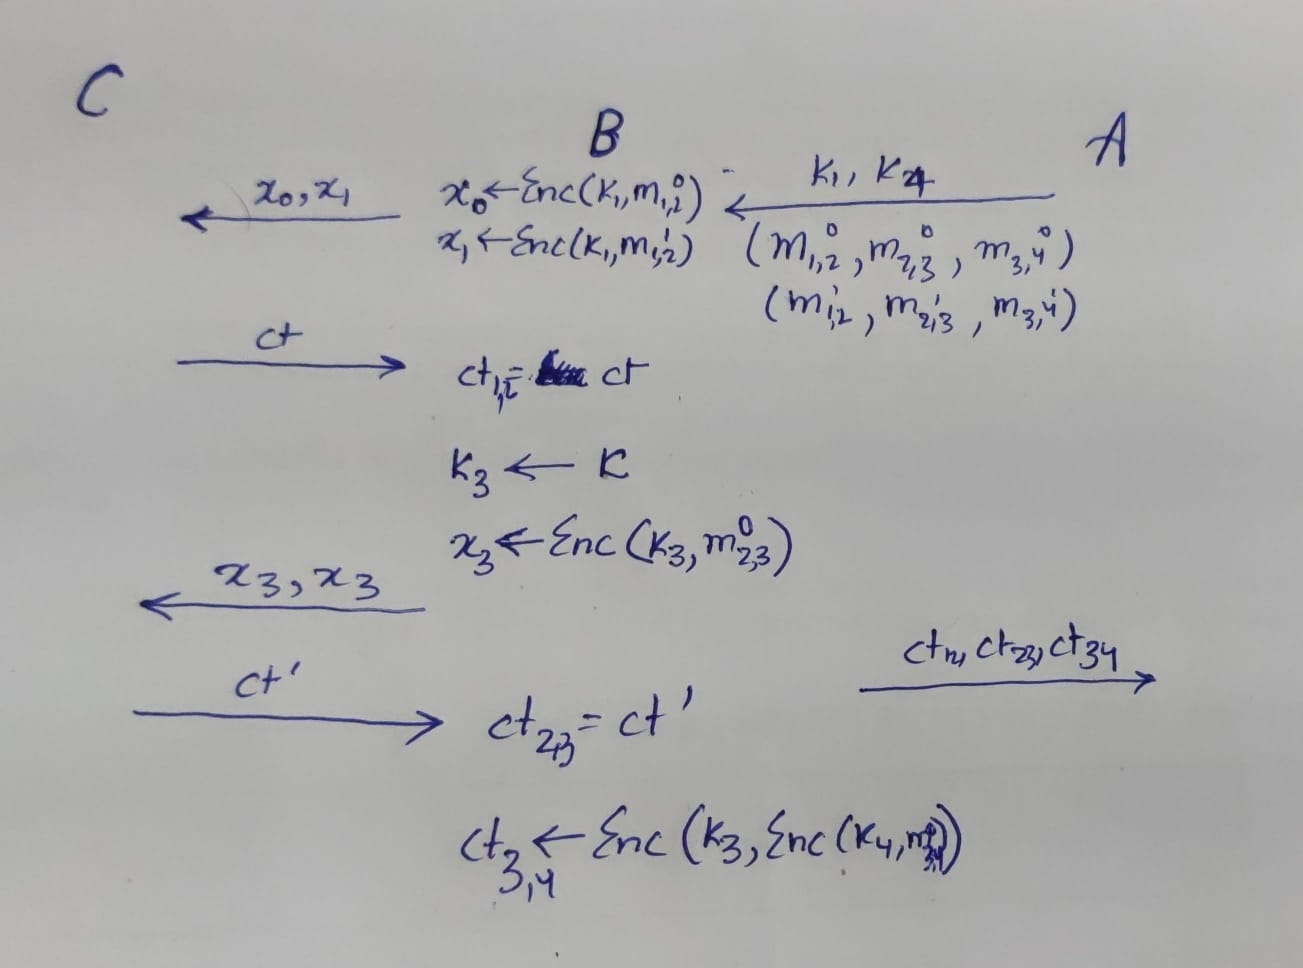
\includegraphics[scale=0.25]{images/Reduction21.jpg}
        \caption{Reduction 1 for Problem 2}
        \label{fig:p21}
    \end{figure}


    \clearpage

    \noindent\textbf{Claim:} If there exists an adversary $\calA$ for which $|p_{\hyb,0}-p_{\hyb,1}|$ is non-negligible then there exists an adversary $\calB$ which breaks the CPA security of $\calE=(\enc,\dec)$ with advantage $|p_{\hyb,0}-p_{\hyb,1}|$


    Consider the reduction \cref{red:p22}:
    \securitygame{Reduction}{Reduction 2 for Problem 2}{\label{red:p22}}
    {
        \begin{itemize}
            \item $\calA$ sends $k_1, k_4$, as well as challenge messages $(m^0_{1,2}, m^0_{2,3},m^0_{3,4})$ and $(m^1_{1,2}, m^1_{2,3},m^1_{3,4})$ to $\calB$
            \item $\calB$ samples $k_2\gets\calK$ and computes $\ct_{1,2}\gets\enc(k_2,\enc(k_1,m^1_{1,2}))$.
            \item $\calB$ sends $m^0_{2,3}, m^1_{2,3}$ to $\calC$ to obtain $\ct=\enc(k_3,m_{2,3}^b)$ and sets $\ct_{2,3}\gets\enc(k_2,\ct)$
            \item $\calB$ computes $x_0\gets\enc(k_4,m_{3,4}^0)$ and sends $(x_0,x_0)$ to $\calC$ to obtain $\ct' = \enc(k_3,\enc(k_4,m^0_{3,4}))$. $\calB$ sets $\ct_{3,4}=\ct'$
            \item $\calB$ sends $(\ct_{1,2}, \ct_{2,3}, \ct_{3,4})$ to $\calA$
            \item For the encryption queries, $\calB$ follows a similar procedure as above.
            \item Finally $\calA$ outputs a bit $b'$ which $\calB$ forwards to $\calC$
        \end{itemize}
    }

    If $\calC$ chooses $b$ to be 0 then the above reduction corresponds to Hybrid World 0  while if he chooses 1, then it corresponds to Hybrid World 1. So the CPA advantage of $\calB=|p_{\hyb,0}-p_{\hyb,1}|$
    \begin{figure}[!ht]
        \centering
        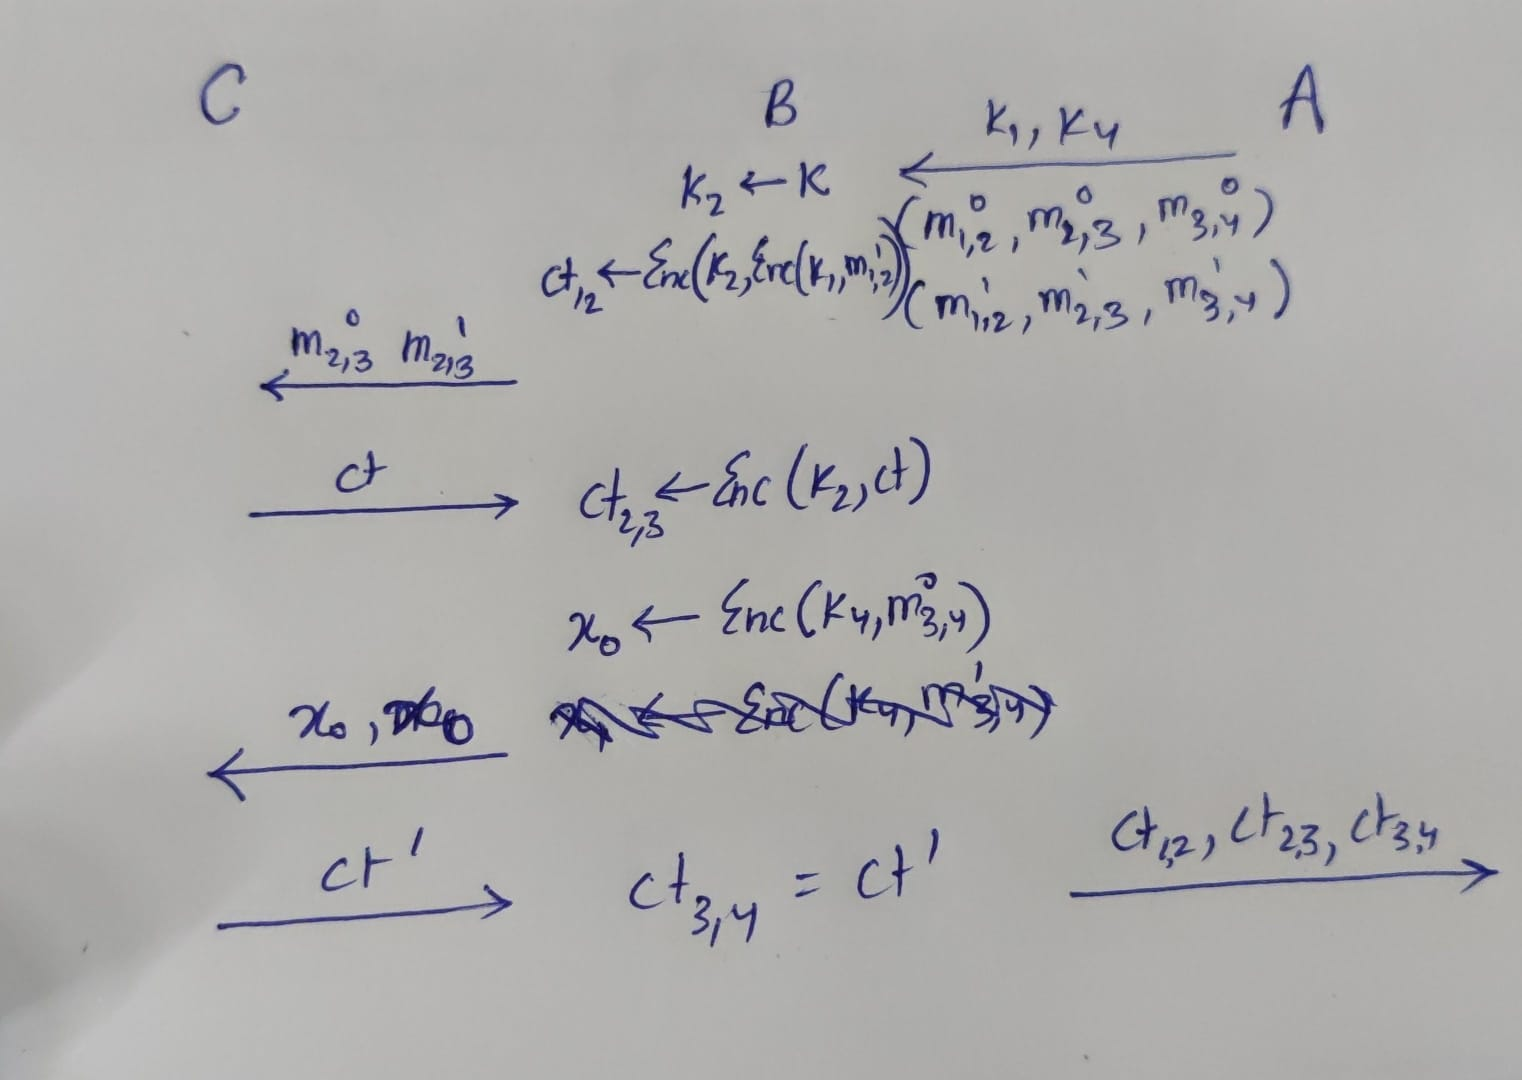
\includegraphics[scale=0.25]{images/Reduction22.jpg}
        \caption{Reduction 2 for Problem 2}
        \label{fig:p22}
    \end{figure}

    \clearpage

    \noindent\textbf{Claim:} If there exists an adversary $\calA$ for which $|p_{\hyb,1}-p_1|$ is non-negligible then there exists an adversary $\calB$ which breaks the CPA security of $\calE=(\enc,\dec)$ with advantage $|p_{\hyb,1}-p_1|$


    Consider the reduction:
    \securitygame{Reduction}{Reduction 3 for Problem 2}{\label{red:p23}}
    {
        \begin{itemize}
            \item $\calA$ sends $k_1, k_4$, as well as challenge messages $(m^0_{1,2}, m^0_{2,3},m^0_{3,4})$ and $(m^1_{1,2}, m^1_{2,3},m^1_{3,4})$ to $\calB$
            \item $\calB$ samples $k_2\gets\calK$ and computes $\ct_{1,2}\gets\enc(k_2,\enc(k_1,m^1_{1,2}))$.
            \item $\calB$ sends $m^1_{2,3}, m^1_{2,3}$ to $\calC$ to obtain $\ct=\enc(k_3,m_{2,3}^1)$ and sets $\ct_{2,3}\gets\enc(k_2,\ct)$
            \item $\calB$ computes $x_0\gets\enc(k_4,m_{3,4}^0), x_1\gets\enc(k_4,m_{3,4}^1)$ and sends $(x_0,x_1)$ to $\calC$ to obtain $\ct' = \enc(k_3,\enc(k_4,m^b_{3,4}))$. $\calB$ sets $\ct_{3,4}=\ct'$
            \item $\calB$ sends $(\ct_{1,2}, \ct_{2,3}, \ct_{3,4})$ to $\calA$
            \item For the encryption queries, $\calB$ follows a similar procedure as above.
            \item Finally $\calA$ outputs a bit $b'$ which $\calB$ forwards to $\calC$
        \end{itemize}
    }

    If $\calC$ chooses $b$ to be 0 then the above reduction corresponds to Hybrid World 1  while if he chooses 1, then it corresponds to World 1. So the CPA advantage of $\calB=|p_{\hyb,1}-p_{1}|$

    \begin{figure}[!ht]
        \centering
        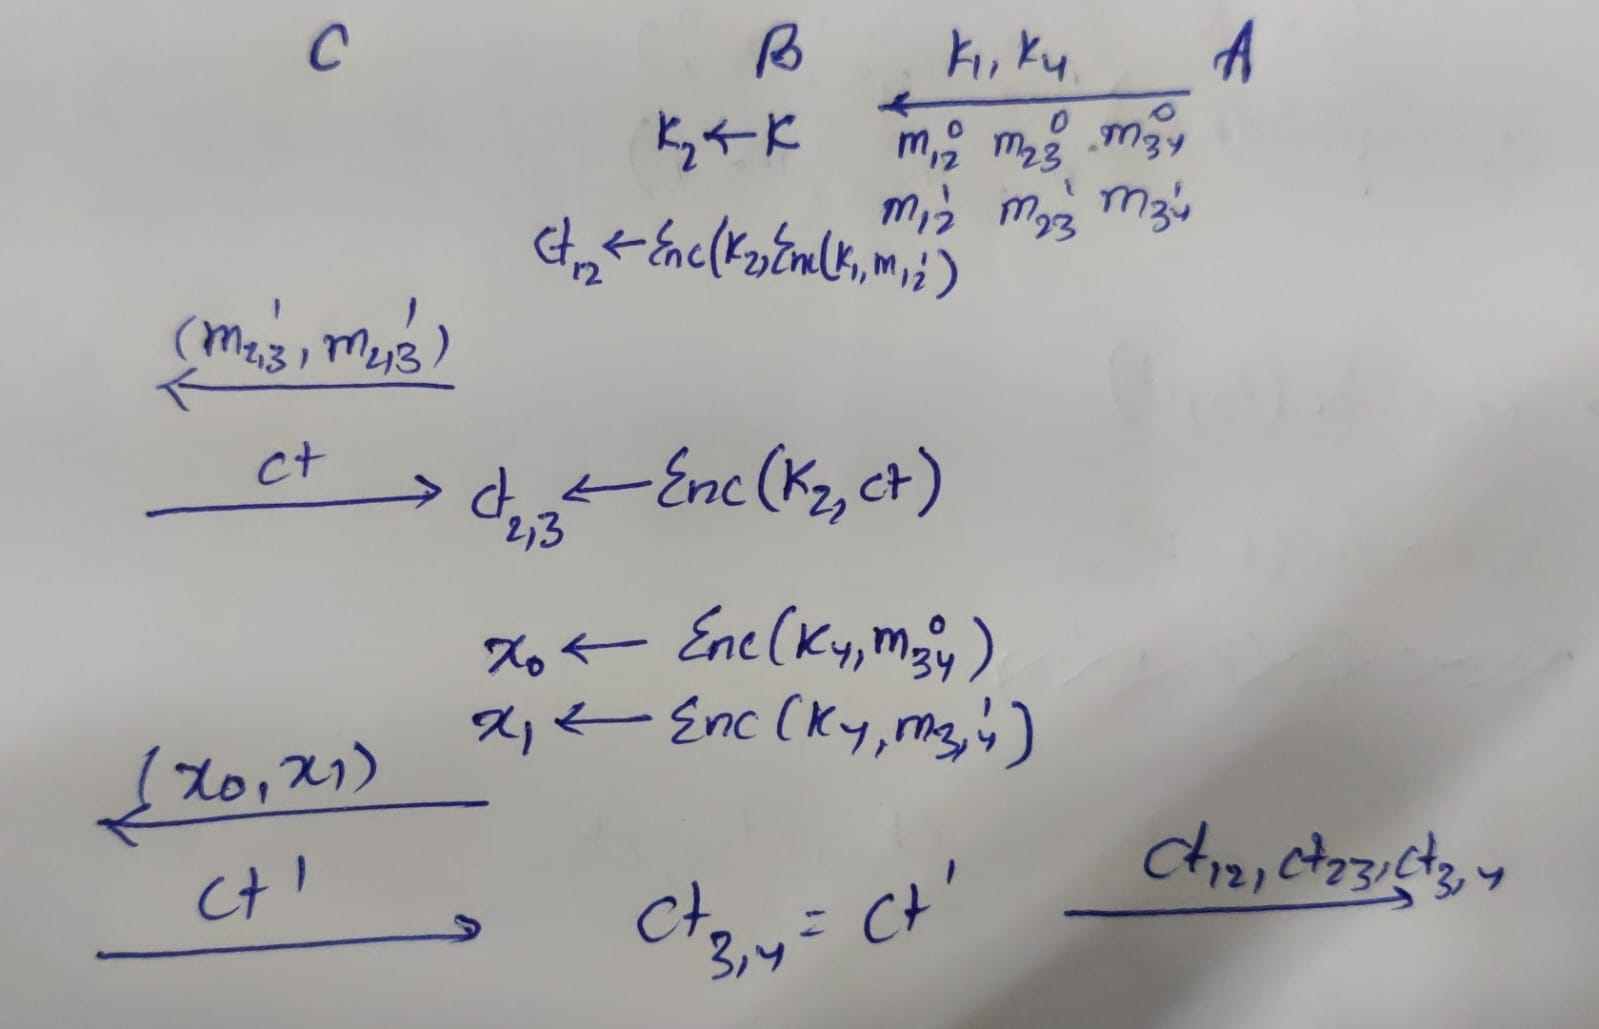
\includegraphics[scale=0.25]{images/Reduction23.jpg}
        \caption{Reduction 3 for Problem 2}
        \label{fig:p23}
    \end{figure}

    Thus from the above three claims, we can conclude that if $(\enc,\dec)$ is CPA secure, then no p.p.t. adversary has non-negligible advantage in the security game defined above.
\end{solution}

\prob{3 : One-time secure MACs, and Upgrading One-Time MACs to Many-Time MACs}
\begin{solution}
    \begin{enumerate}[(a)]
        \item We construct the following One-Query Unconditionally Secure MAC scheme $\calI = (\sign, \verif)$ :
              $$\sign(k, m) = (m \wedge k_1) \vee k_2$$ and
              $$\verif(k, m, \sigma) = \begin{cases}
                      1 & \text{if } \sigma =  (m \wedge k_1) \vee k_2 \\
                      0 & \text{Otherwise}
                  \end{cases}$$
              where $k = (k_1, k_2)$ is sampled from keyspace $\calK = \bit^{2n}$ ($k_1$ and $k_2$ are n bits each). Also the signature space is $\bit^n$. \\ \\
              \textbf{Claim :} The winning probability of an computationally unbounded adversary $\calA$ is bounded by $\frac{1}{2^n}$, and hence is negligible.
              \begin{proof} On getting the signature of some message $m \in \calM$, the adversary knows $m$, $\sigma$ and $n$ but doesn't know $(k_1, k_2)$. So if the adversary enumerates all such possible pairs of $(k_1, k_2)$ which satisfies this equation, then there are about $2^n$ such pairs. \\
              To prove this, consider the $i^{th}$ bit of message m ($m_i$) and corresponding bit in $\sigma$ ($\sigma_i$). Also take $i^{th}$ bits of $k_1$ and $k_2$ as $a_1$ and $a_2$. \\
              \textbf{Case 1:} $m_i = 0$ and $\sigma_i = 0$ \\
              \textit{Possibilities:} for $a_1 = 0$, $a_2$ can only be 0 and for $a_1 = 1$, $a_2$ can be only 0. (2 pairs of $(k_1, k_2)$)\\
              \textbf{Case 2:} $m_i = 0$ and $\sigma_i = 1$ \\
              \textit{Possibilities:} for $a_1 = 0$, $a_2$ can only be 1 and for $a_1 = 1$, $a_2$ can be only 1. (2 pairs of $(k_1, k_2)$)\\
              \textbf{Case 3:} $m_i = 1$ and $\sigma_i = 1$ \\
              \textit{Possibilities:} for $a_1 = 0$, $a_2$ can only be 1 and for $a_1 = 1$, $a_2$ can be both 0 and 1. (3 pairs of $(k_1, k_2)$)\\
              \textbf{Case 4:} $m_i = 1$ and $\sigma_i = 0$ \\
              \textit{Possibilities:} for $a_1 = 0$, $a_2$ can only be 0 and for $a_1 = 1$, there is no possible value of $a_2$. (1 pair of $(k_1, k_2)$)\\
              So overall there are $2^n$ expected number of pairs of $k_1$ and $k_2$ satisfying our equation. \\ \\
              Now if the adversary wants to send forgery $\sigma'$ of some different message $m'$, such that $\sigma' = (k_{i1} \wedge m') \vee k_{i2}$, where $k_{i1}$ is some choice of key $k_1$ by $\calA$ and $k_{i2}$ is the corresponding key $k_2$ which satisfies $\sigma = (m \wedge k_{i1}) \vee k_{i2}$. But for different choices of $k_{i1}$, the corresponding $\sigma'$ is different. So there are $2^n$ different equally likely choices of $\sigma'$ which the adversary can send as forgery out of which only one is correct.\\
              \end{proof}
              Hence our one-query Unconditionally Secure MAC is secure even against an unbounded adversary.

        \item To prove the security of our MAC scheme $\calI = (\sign, \verif)$, we setup the following games : \\ \\
              \textbf{Game 0:} This is the usual MAC security game.
              \begin{itemize}
                  \item \textbf{Setup Phase :} Challenger chooses a PRF key $k = (k_1, k_2)$ where $k_1 \epsilon \calK_1$ and $k_2 \epsilon \calK_2$.
                  \item \textbf{Query Phase :} Adversary sends polynomially many queries. For the $i^{th}$ query $m_i$, the challenger chooses a random string $r_i \leftarrow \calX$ and sends $\sigma_i = \sign(k, m_i ; r_i)$ to the adversary.
                  \item \textbf{Forgery :} Finally, the adversary outputs $(m^*, \sigma^*)$ such that $(m^*, \sigma^*) \neq (m_i, \sigma_i)$ for all i.
              \end{itemize}

              Let the winning probability of Adversary $\calA$ in Game 0 be $p_0$. \\ \\
              \textbf{Game 1:} This is similar to previous game except the PRF is replaced by a uniformly random function.
              \begin{itemize}
                  \item \textbf{Setup Phase :} Challenger chooses a PRF key $k = (k_1, k_2)$ where $k_1 \epsilon \calK_1$ and $k_2 \epsilon \calK_2$. It also samples a unifromly random function $f \leftarrow Func[\calX, \calT]$.
                  \item \textbf{Query Phase :} Adversary sends polynomially many queries. For the $i^{th}$ query $m_i$, the challenger chooses a random string $r_i \leftarrow \calX$ and sends $\sigma_i = (r, \sign_1(k_1, m_i) \oplus f(r_i))$ to the adversary.
                  \item \textbf{Forgery :} Finally, the adversary outputs $(m^*, \sigma^*)$ such that $(m^*, \sigma^*) \neq (m_i, \sigma_i)$ for all i.
              \end{itemize}
              Let the winning probability of Adversary $\calA$ in Game 1 be $p_1$. \\ \\
              \textbf{Game 2:} This is similar to previous game except the signature is replaced by a uniformly random function.
              \begin{itemize}
                  \item \textbf{Setup Phase :} Challenger chooses a PRF key $k = (k_1, k_2)$ where $k_1 \epsilon \calK_1$ and $k_2 \epsilon \calK_2$. It also samples two uniformly random functions $f \leftarrow Func[\calX, \calT]$ and $f' \leftarrow Func[\calM, \calT]$.
                  \item \textbf{Query Phase :} Adversary sends polynomially many queries. For the $i^{th}$ query $m_i$, the challenger chooses a random string $r_i \leftarrow \calX$ and sends $\sigma_i = (r, f'(m_i) \oplus f(r_i))$ to the adversary.
                  \item \textbf{Forgery :} Finally, the adversary outputs $(m^*, \sigma^*)$ such that $(m^*, \sigma^*) \neq (m_i, \sigma_i)$ for all i.
              \end{itemize}
              Let the winning probability of Adversary $\calA$ in Game 2 be $p_2$. \\ \\
              \textbf{Claim 1:} $p_2 = \epsilon$, where $\epsilon$ is a negligible function. \\
              \textit{Proof:} This is because $f$ and $f'$ are truly random functions and the adversary can never predict the output of these functions at some input (Using Shannon's security). It can only guess the output with a probability of $\frac{1}{|\calT|}$. So the value of $p_2$ is negligible. \\ \\
              \textbf{Claim 2:} $|p_1 - p_0|$ is negligible. \\
              \textit{Proof:} This follows from the security of the PRF function. Suppose there exists an adversary $\calA$ that can distinguish between the two games (i.e. $|p_1 - p_0|$ is non-negligible), then we can construct a reduction $\calB$ which uses this adversary to win the PRF game with non-negligible advantage.
              The reduction works as follows:
              \begin{itemize}
                  \item It samples $r_i \leftarrow \calX$ for the $i^{th}$ query. It sends this to the PRF challenger and receives $y_i$.
                  \item It then sends $(r_i, y_i \oplus \sign_1(k_1, m))$ to the adversary. The adversary finally outputs a forgery $(m^*, \sigma^*)$, where $\sigma^* = (\sigma^*_0, \sigma^*_1)$
                  \item The reduction then sends a final query $\sigma^*_0$ to the PRF challenger and receives $y^*$. If $y^* = \sigma^*_1 \oplus \sign_1(k_1, m^*)$ then the reduction sends 1, else it sends 0.
              \end{itemize}
              If the PRF challenger chooses pseudorandom, then the reduction will output 0 with a probability of $p_0$ else if the PRF challenger chooses completely random function, then the reduction sends 1 with probability $p_1$.\\
              Hence the $\mathsf{PRFAdv}[\calB, \calF] = |p_0 - p_1|$, which is negligible.
              \\ \\
              \textbf{Claim 3:} $|p_2 - p_1|$ is also negligible. \\
              \textit{Proof:} Suppose in game 1, the adversary sends a forgery as $(m^*, \sigma^*)$. We can then write $p_1$ as follows: \\
              $p_1 = \Pr[\text{A wins game 1 and A also knows $\sign_1(k_1, m^*)$}] +$ \\
              $\Pr[\text{A wins game 1 and A doesn't know $\sign_1(k_1, m^*)$}]$
              \\
              The second case (A wins game 1 but A doesn't know $\sign_1(k_1, m^*)$) is equivalent to game 2, since A doesn't was not able to compute the function, $\sigma_1$ behaves as a random function for the adversary. So we can write :
              $$|p_1 - p_2| = \Pr[\text{A wins game 1 and A also knows $\sign_1(k_1, m^*)$}]$$ and from this ,
              $$|p_1 - p_2| \leq \Pr[\text{A knows }\sign_1(k_1, m^*)]$$
              Now we can say that the above term is negligible using one-query security of $\sigma_1$. This is because in all the queries of the adversary, we sent the signature as $f(r) \oplus \sigma_1$ where $f(r)$ is some truly random function. Using Shannon's OTP security, we can say that $f(r) \oplus \sigma_1$ is also completely random to the adversary. So the probability that adversary sends $\sign_1(k_1, m^*)$ without knowing the signature of any other message $m \epsilon \calM$ is negligible because $\sigma_1$ is one-query secure. \\ \\
              Hence using all the above three claims, we can say that $p_0$ is negligible and hence our MAC scheme $\calI$ is secure.

    \end{enumerate}
\end{solution}


\prob{4 : CCA Security v/s Authenticated Encryption}
\begin{solution}
    \begin{enumerate}[(a)]
        \item Here we need to show that CCA+PT-INT $\implies$ CT-INT. Intuitively, this is true because if an adversary breaks CT-INT, he produces a ciphertext of (1) a previously queried message or (2) a new message. If (1) happens then CCA breaks and if (2) happens then PT-INT breaks.

              Let $\calE=(\enc,\dec)$ be an encryption scheme that follows CCA and PT-INT. We will show that it satisfies CT-INT. Consider the following worlds:
              \begin{world}[World 0:]
                  This is the CT-INT game
              \end{world}

              \begin{world}[Hybrid Word]
                  This is the CT-INT game but the $\ct^*$ given as output by the adversary decripts to one of the previously queried messages: $\dec(k,\ct^*)\in\{m_i\}$
              \end{world}

              Let $p_0$ and $p_\hyb$ be the winning probabilities of the adversary in World 0 and Hybrid World respectively.

              \textbf{Claim:} If there exists an adversary for which $|p_0-p_\hyb|$ is non-negligible then there exists a reduction $\calB$ which breaks the PT-INT of $\calE$
              \begin{proof}
                  Indeed, if $p_0$ and $p_\hyb$ are far apart then the probability that the output $\ct^*$ given by $\calA$ decrypts to a message different from the queried messages is non-negligible. This is sufficient to break PT-INT. The reduction simply forwards $\ct^*$ and wins with probability $|p_0-p_\hyb|$
              \end{proof}

              \textbf{Claim:} If there exists an adversary for which $p_\hyb$ is non-negligible then there exists a reduction $\calB$ which breaks the CCA security of $\calE$
              \begin{proof}
                  Consider the following reduction:
                  \securitygame{Reduction}{Reduction for Problem 4a}{\label{red:p4a}}
                  {
                      \begin{itemize}
                          \item $\calA$ sends $m_i$ to $\calB$
                          \item $\calB$ samples $m\gets\calM$ and sends encryption query $(m_i,m)$ to CCA challenger $\calC$
                          \item $\calC$ replies with $\ct_i$ which $\calB$ forwards to $\calA$
                          \item Finally, $\calA$ outputs $\ct^*$ which $\calB$ forwards to $\calC$ for decryption. If the output is $\perp$, $\calB$ outputs 1 otherwise it outputs 0
                      \end{itemize}
                  }

                  Let the number of queries made by $\calA$ be $Q$ and the message space be $\calM$.

                  Now, if the challenger chooses $b=0$ then it is the same as the CT-INT game.  $$\Pr[b'=0|b=0]=p_\hyb$$
                  If challenger choose $b=1$ then for all its queries, $\calA$ gets the encryption of a random message $m$. The probability of outputing 0 here will be bounded by the probability that $m\in\{m_i\}$ which is
                  $$\Pr[\exists m_i : m=m_i]\leq\frac{Q}{|\calM|}$$
                  Thus, $$\Pr[b'=0|b=1]\leq \frac{Q}{|\calM|}$$
                  $$\mathsf{CCAAdv}[\calB, \calC]\geq p_\hyb-\frac{Q}{|\calM|}$$
                  Which is non-negligible assuming $\calM$ to be superpolynomial.
              \end{proof}
        \item We use \textbf{Strong PRP}\footnote{ This can be created by using a 4-round Luby-Rakoff Construction. A strong PRP is secure against inversion queries too} $P_s$ as the cryptographic primitive in our scheme $\calE=(\enc,\dec)$.

              $$\enc(k,m):=\{r\gets\calR, \ct\gets P_s(k,(m,r)),\text{Output } \ct\}$$
              $$\dec(k,\ct):=\{(m,r)=P_s^{-1}(k,\ct), \text{Output } m\}$$

              Observe that if the ciphertexts are tampered with, they will still get decrypted to some message $m'$ since the decryption algorithm never outputs abort. Hence, this scheme \textbf{doesn't satisfy plaintext integrity}.

              % However, the adversary cannot use decryption queries to his advantage in the CCA security game. For this purpose, he should be able to tamper with the ciphertext and produce a valid encryption of a message he can \textit{predict}. We claim that this prediction will not be possible, as formalized in the proof below:

              \textbf{Claim:} $\calE$ is CCA secure
              \begin{proof}
                  We will show the CCA security of our encryption scheme using hybrid worlds as follows:
                  \begin{world}[World-b]
                      \begin{itemize}
                          \item This is the usual CCA game. The challenger samples a key $k \leftarrow \calK$, a bit $b \leftarrow \bit$ and a random string $r \leftarrow \calR$.
                          \item For the $i^{th}$ Encryption query of the adversary $(m_{i0}, m_{i1})$, the challenger forwards $\enc(k, m_{ib})$ to the adversary.
                          \item For the $j^{th}$ Decryption query of the adversary $(\ct_{j})$, the challenger calculates $(m_j, r_j) \leftarrow \dec(k, \ct_j)$ and sends $m_j$ to the adversary.
                          \item After polynomially many queries, the adversary finally outputs its guess bit $b'$.
                      \end{itemize}
                      Let $\Pr[b' = 0] = p_b$
                  \end{world}

                  \begin{world}[Hybrid-World-b]
                      \begin{itemize}
                          \item This is the usual CCA game except know the challenger uses purely random permutations. The challenger samples a bit $b \leftarrow \bit$, a random string $r \leftarrow \calR$ and a uniformly random permutation $f \leftarrow Perm[\calM]$.
                          \item For the $i^{th}$ Encryption query of the adversary $(m_{i0}, m_{i1})$, the challenger forwards $f(m_{ib}||r)$ to the adversary.
                          \item For the $j^{th}$ Decryption query of the adversary $(\ct_{j})$, the challenger computes $(m_j, r_j) \leftarrow f^{-1}(\ct_j)$ and forwards $m_j$ to the adversary.
                          \item After polynomially many queries, the adversary finally outputs its guess bit $b'$.
                      \end{itemize}
                      Let $\Pr[b' = 0] = p_{\hyb\_b}$
                  \end{world}

                  \textbf{Claim 1:} $p_{\hyb\_0} = p_{\hyb\_1}$. \\
                  \textit{Proof:} This follows from the fact that the challenger uses a purely random permutation $f(.)$ to calculate the encryption. So, using Shannon's security, the adversary cannot distinguish between the two hybrid worlds even by knowing the previous encryption and decryption queries. \\ \\

                  \textbf{Claim 2:} $|p_{\hyb\_b} - p_b|$ is negligible. \\
                  \textit{Proof:} Suppose that there exists an adversary $\calA$ that can distinguish between World-b and Hybrid-world-b. We can then create a reduction $\calB$ such that it breaks the strong PRP security with non-negligible advantage using the adversary $\calA$.\\
                  The reduction works as follows:
                  \begin{itemize}
                      \item The reduction takes all the encryption queries from the adversary and forwards them to the PRP challenger as forward queries. It then forwards the replies from the challenger back to the adversary.
                      \item Similarly, the reduction takes all the decryption queries from the adversary and forwards them to the PRP challenger as inversion queries. It then forwards the replies from the challenger back to the adversary.
                      \item After polynomially many queries, the adversary $\calA$ sends a bit $b'$ to the reduction. The reduction sends the bit $b'$ as its guess to the strong PRP challenger.
                  \end{itemize}
                  Here if the PRP challenger chooses to send psuedorandom permutations, then that corresponds to World-b for the adversary and it sends $b' = 0$ with a probability of $p_b$. On the other hand, if the PRP challenger sends truly random permutations that correspond to Hybrid-World-b for the adversary and it sends $b' = 1$ with a probability of $p_1$. \\
                  The $\mathsf{PRPAdv}[\calB, P_s] = |p_{\hyb\_b} - p_b|$. Hence $|p_{\hyb\_b} - p_b|$ must be negligible.\\ \\
                  Using the above two claims, we can say that $|p_0 - p_1|$ is negligible and hence our encryption scheme is CCA secure.
                  \\ \\
              \end{proof}
              
    \end{enumerate}

\end{solution}

\prob{5: Modular Arithmetic and Basic Group Theory}
\begin{solution}
    \begin{enumerate}[(a)]
        \item Since $a$ and $p$ are coprime, by the Extended Euclid's Agorithm:
              $$ ab+py=\gcd(a,p)=1    $$
              Taking modulo p on both sides:
              $$ ab \mod p =1    $$
              Where $b\in\Z_p$ (If not then by the division algorithm $b=qp+b', b'<p$. So, we can replace $b$ with $b'$)
              \vspace{20pt}

              Now suppose there exist $b, b'\in\Z_p$ such that
              $$ ab=1\mod p \hspace{50pt} ab'=1\mod p    $$
              Then by definition of mod, $p|a(b-b')$. So $b-b'=0$ since $a$ and $b-b'$ will be coprime to $p$. Hence $b$ is unique.

        \item Consider $h(y)=y^2+y$ and $n=6$. For 3 values of $y$ viz. $2,3,5$, we have $h(y)=0\mod 6$. Thus
              $$|\{y\in\Z_6:y^2+y=0\mod6\}|=3>2$$

        \item For this part, we will use Fermat's Little Theorem.
              \begin{theorem}[Fermat's Little Theorem]
                  For any prime number $p$ and $a\in\Z$
                  $$a^{p-1}=1\mod p$$
              \end{theorem}
              \begin{proof}
                  We use the following observation:

                  \textbf{Observation:} Let $a \in\Z^*_p$. Consider the set $S_a = \{a\cdot i: i\in\Z^*_p\}$. Then $S_a = \Z^*_p$.

                  Otherwise, suppose there exist $i,j\in\Z^*_p$ such that $$a\cdot i \mod p= a\cdot j\mod p\implies p | a (i-j)\implies i=j$$

                  Now consider the product of all elements of $S_a$

                  $$\prod_{a_i\in S_a}a_i=\prod_{i=1}^{p-1}a\cdot i=a^{p-1}\prod_{i\in\Z^*_p}i$$
                  Since $S_a = \Z^*_p$, the products on both sides must be the same. Hence $$a^{p-1}=1\mod p$$


              \end{proof}
              Let $a\in\Z_p$ and $r=\ord(a)$. Then $a^r=1\mod p$. By Fermat's Little Theorem:
              $$a^{p-1}=1\mod p$$
              Suppose by the division algorithm, $p-1=rq+s$, $s<r$. Since $a^{p-1}=1\mod p$ and $a^{r}=1\mod p$, $$a^{p-1-rq}=1\mod p$$ and hence $a^{s}=1\mod p$. But since $s<r$, $s$ must be 0.

        \item The reduction works as \cref{red:p5d}
        \securitygame{Reduction}{Reduction for Problem 5d}{\label{red:p5d}}
        {
              \begin{itemize}
                \item The challenger samples $\alpha,\beta,\gamma\gets\Z_q, b\gets\bit$ and calculates $u=g^\alpha, v_0=g^{\alpha^2},v_1=g^\beta, w_0=g^{\alpha^3}, w_1=g^\gamma$ and sends $(g, u, v_b, w_b)$ to $\calB$
                \item $\calB$ samples $\delta\gets\Z_q$ and sends $(g, u, v_bg^\delta, w_bu^\delta)$ to $\calA$
                \item $\calA$ returns a bit $b'$ which $\calB$ forwards to $\calC$
              \end{itemize}
        }

        If $b=0$ $\calA$ gets $(g, g^\alpha, g^{\alpha^2+\delta}, g^{\alpha(\alpha^2+\delta)})$ which is of the form $(g, g^\alpha, g^{\beta'}, g^{\alpha\beta'})$ since $\delta$ is chosen at random. Hence the distribution reduces to the DDH distribution $\calD'=\{(g,g^\alpha,g^\beta, g^{\alpha\beta}): \alpha,\beta,\gamma\gets\Z_q\}$

        If $b=1$ $\calA$ gets $(g, g^\alpha, g^{\beta+\delta}, g^{\gamma+\alpha\delta})$ which is of the form $(g, g^\alpha, g^{\beta'}, g^{\gamma'})$ since $\beta, \delta$ are chosen at random.

       
        

              \begin{figure}[!ht]
                  \centering
                  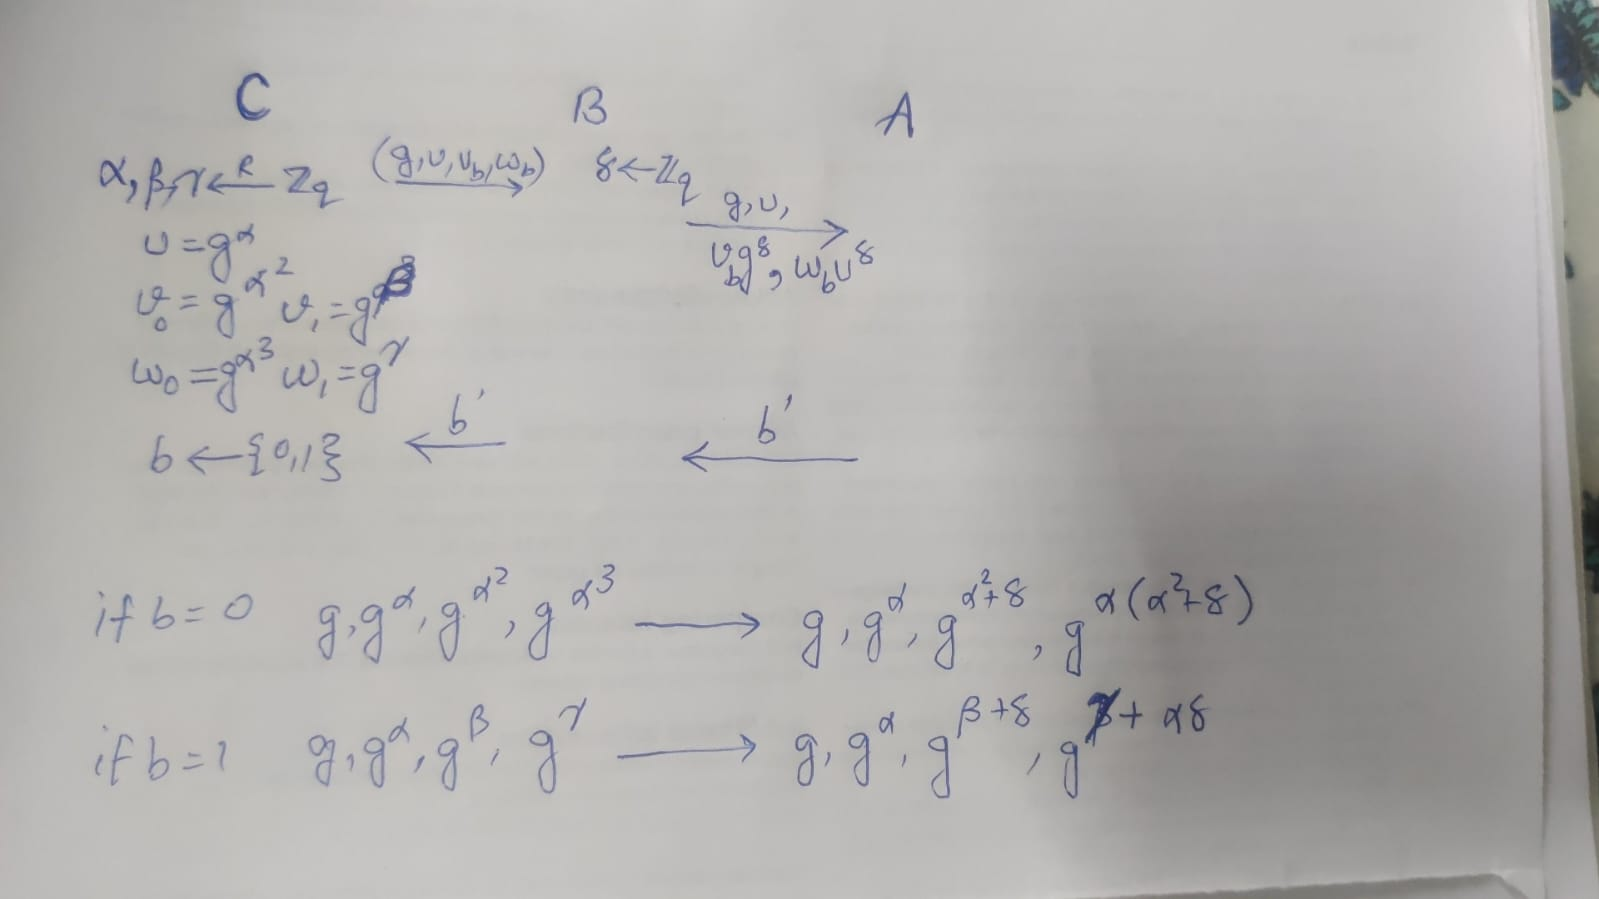
\includegraphics[scale=0.25]{images/Reduction5d.jpg}
                  \caption{Reduction for Problem 5d}
                  \label{fig:p5d}
              \end{figure}

        \item Let $S_i$ denote the set of matrices $M\in\Z_q^{t\times t}$ where the last $i$ rows are of the form
              $$\lambda_j (v_1 \dots v_t),\hspace{20pt} j\in[i], (v_1 \dots v_t)\gets\Z_q^t, \lambda_j\gets\Z_q$$

              and the remaining rows have elements sampled at random from $\Z_q$. In other words, last $i$ rows are random multiples of some tuple (chosen at random) and remaining rows are drawn at random. Observe that $S_n=\mathsf{Rank}_1[t,q]$ and $S_1=\Z_q^{t\times t}$.

              The proof proceedes by a sequence of $n$ hybrid worlds:
              \begin{world}[Hybrid World $\mathbf{i}$:]
                  The Challenger samples from the distribution $$\calD'_i=\{(g,g^\mathbf{M}): g\gets G,\mathbf{M}\gets S_i \}$$
              \end{world}
              Observe that Hybrid World 1 corresponds to sampling from $\calD_1$ and Hybrid World $n$ corresponds to sampling from  $\calD_0$ specified in the question.
              Let $p_i$ be the probability of the Adversary outputting 0 in the above Hybrids.

              \textbf{Claim:} If there exists an adversary $\calA$ such that $|p_i-p_{i+1}|$ is non-negligible then there exists an adversary $\calB$ which solves the DDH problem for group $G$.

              \begin{proof}
                  Consider the following reduction:


                  \securitygame{Reduction}{Reduction for Problem 5e}{\label{red:p5e}}
                  {
                      \begin{itemize}
                          \item $\calC$ samples $b\gets\bit$ and $g\gets G$. He calculates $g^\alpha, g^\beta$ and $w_0=g^{\alpha\cdot\beta}, w_1=g^\gamma$ where $\alpha,\beta,\gamma\gets\Z_q$ and sends $(g, g^\alpha, g^\beta, w_b)$ th $\calB$
                          \item $\calB$ samples the following:
                                $$\beta_1,\beta_2,\dots\beta_{t-1}\gets\Z_q$$
                                $$\lambda_1,\lambda_2,\dots\lambda_{i}\gets\Z_q$$
                                $$v_{i,j}\gets\Z_q\hspace{20pt}1\leq i\leq {t-i-1}, 1\leq j \leq t$$
                                And computes the matrix:
                                $$
                                    \begin{bmatrix}
                                        g^{v_{1,1}}        & g^{v_{1,2}}          & \dots  & g^{v_{1,t}}              \\
                                        \vdots             & \vdots               & \ddots & \vdots                   \\
                                        g^{v_{t-i-1,1}}    & g^{v_{t-i-1,2}}      & \dots  & g^{v_{t-i-1,t}}          \\
                                        w_b                & g^{\alpha\beta_1}    & \dots  & g^{\alpha\beta_{t-1}}    \\
                                        g^{\lambda_i\beta} & g^{\lambda_i\beta_1} & \dots  & g^{\lambda_i\beta_{t-1}} \\
                                        \vdots             & \vdots               & \ddots & \vdots                   \\
                                        g^{\lambda_1\beta} & g^{\lambda_1\beta_1} & \dots  & g^{\lambda_1\beta_{t-1}}
                                    \end{bmatrix}
                                $$
                                And sends it to $\calA$

                          \item $\calA$ responds with a bit $b'$ which $\calB$ forwards to $\calC$
                      \end{itemize}
                  }

                  \begin{figure}[!ht]
                      \centering
                      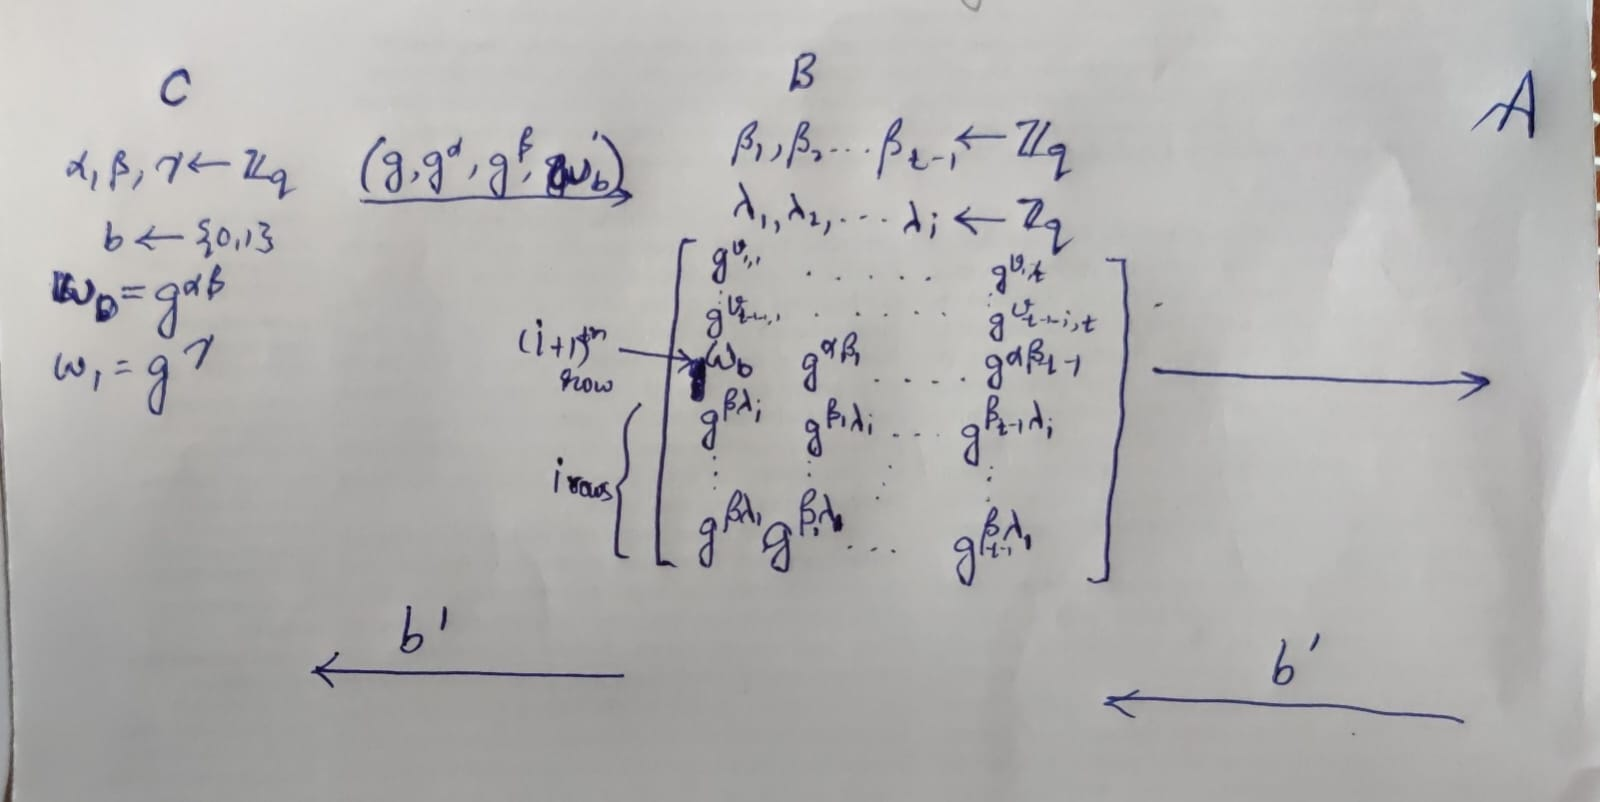
\includegraphics[scale=0.25]{images/Reduction5e.jpg}
                      \caption{Reduction for Problem 5e}
                      \label{fig:p5e}
                  \end{figure}

                  Observe that if $b=0$ then it corresponds to Hybrid World $i+1$ and if $b=1$ then it corresponds to Hybrid World $i$. This is because the matrix
                  $$
                      \begin{bmatrix}
                          {v_{1,1}}        & {v_{1,2}}          & \dots  & {v_{1,t}}              \\
                          \vdots           & \vdots             & \ddots & \vdots                 \\
                          {v_{t-i-1,1}}    & {v_{t-i-1,2}}      & \dots  & {v_{t-i-1,t}}          \\
                          \alpha\beta      & {\alpha\beta_1}    & \dots  & {\alpha\beta_{t-1}}    \\
                          {\lambda_i\beta} & {\lambda_i\beta_1} & \dots  & {\lambda_i\beta_{t-1}} \\
                          \vdots           & \vdots             & \ddots & \vdots                 \\
                          {\lambda_1\beta} & {\lambda_1\beta_1} & \dots  & {\lambda_1\beta_{t-1}}
                      \end{bmatrix}
                  $$
                  Has the last $i+1$ rows as the multiple of the tuple $(\beta, \beta_1, \beta_2\dots\beta_{t-1})$ while
                  $$
                      \begin{bmatrix}
                          {v_{1,1}}        & {v_{1,2}}          & \dots  & {v_{1,t}}              \\
                          \vdots           & \vdots             & \ddots & \vdots                 \\
                          {v_{t-i-1,1}}    & {v_{t-i-1,2}}      & \dots  & {v_{t-i-1,t}}          \\
                          \gamma           & {\alpha\beta_1}    & \dots  & {\alpha\beta_{t-1}}    \\
                          {\lambda_i\beta} & {\lambda_i\beta_1} & \dots  & {\lambda_i\beta_{t-1}} \\
                          \vdots           & \vdots             & \ddots & \vdots                 \\
                          {\lambda_1\beta} & {\lambda_1\beta_1} & \dots  & {\lambda_1\beta_{t-1}}
                      \end{bmatrix}
                  $$
                  Has the last $i$ rows as the multiple of the tuple $(\beta, \beta_1, \beta_2\dots\beta_{t-1})$. Hence, $$\mathsf{DDHAdv}[\calB, \calC]=|p_i-p_{i+1}|$$
              \end{proof}
              \vspace{20pt}
              Therefore we observe that the hybrid worlds are computationally indistinguishable. Assuming that the DDH problem is hard on $G$,
              $$|p_1-p_{n}|\leq \sum_{i=1}^{n-1}|p_i-p_{i+1}|$$
              Which is negligible assuming $|p_i-p_{i+1}|$ is negligible. So, $\calD_0$ and $\calD_1$ are computationally indistinguishable.



    \end{enumerate}
\end{solution}

\end{document}
